\section{Experiment}
\label{sec:experiments}

In this section, we conduct a series of experiments to answer the following research questions:

\noindent \textbf{RQ1.} How does UniGRec perform in comparison with existing generative recommendation methods?

\noindent \textbf{RQ2.} What is the contribution of each individual component to the overall effectiveness of UniGRec?

\noindent \textbf{RQ3.} How do specific hyperparameters or designs affect the performance of UniGRec?

\noindent \textbf{RQ4.} What are the underlying factors driving the observed performance gains of UniGRec?

\subsection{Experimental Setting}

\begin{table}[t]
\caption{Statistical details of the evaluation datasets, where “AvgLen” is the average length of historical sequences. }
\label{table:datasets}
\begin{tabular}{cccccc}
\hline
Dataset       & \#User & \#Item & \#Interaction & Sparsity & AvgLen \\ \hline
Beauty        & 22362  & 12083  & 198313        & 99.93\%  & 8.87 \\
Pet           & 19855  & 8498   & 157747        & 99.91\%  & 7.95 \\
Upwork        & 15542  & 33508  & 139217        & 99.97\%  & 8.96 \\ \hline
\end{tabular}
\end{table}

\subsubsection{Datasets}

We conduct experiments on three real-world datasets, including two publicly available benchmarks from the Amazon Reviews corpus\footnote{\url{https://jmcauley.ucsd.edu/data/amazon/index_2014.html}} (\textit{Beauty} and \textit{Pet}), and one private production dataset collected from our online freelancing platform (\textit{Upwork}). In the Upwork dataset, each interaction corresponds to a time-stamped employer–freelancer hiring event, where employers are treated as users and freelancers are treated as items. The detailed statistics of all datasets are summarized in Table~\ref{table:datasets}.

Following prior work~\cite{SASRec, TIGER}, we apply a 5-core filtering strategy, retaining only users and items with at least five interactions. Each user’s interaction history is truncated or padded to a fixed length of 20 using the most recent interactions. We adopt a leave-one-out splitting strategy, where the most recent interaction of each user is used for testing, the second most recent for validation, and the remaining interactions for training.

\subsubsection{Baselines}
\label{sec:exp_baselines}

The baseline methods used for comparison fall into the following two categories:

\vspace{+3pt}
(a) \noindent\textit{Traditional recommendation methods:}
\begin{itemize}[leftmargin=*]
    \item \textbf{Caser}~\cite{Caser}: This method leverages both horizontal and vertical convolutional filters to extract sequential patterns from user behavior data, capturing diverse local features.
    \item \textbf{GRU4Rec}~\cite{GRU4Rec}: This method employs recurrent neural network (GRU) for session-based recommendation.
    \item \textbf{SASRec}~\cite{SASRec}: This method leverages the self-attention mechanism in Transformers to capture users’ historical preferences.
    \item \textbf{BERT4Rec}~\cite{BERT4Rec}: This method employs bidirectional self-attention to model user behavior sequences and uses a Cloze objective to predict masked items. 
    \item \textbf{HGN}~\cite{HGN}: This method introduces a hierarchical gating mechanism to adaptively integrate long-term and short-term user preferences derived from historical item sequences.
\end{itemize}

(b) \noindent\textit{Generative recommendation methods:}
\begin{itemize}[leftmargin=*]

    \item \textbf{TIGER}~\cite{TIGER}: This method employs an RQ-VAE to encode item representations into discrete semantic IDs and adopts a generative retrieval paradigm for sequential recommendation.
    
    \item \textbf{LETTER}~\cite{LETTER}: This method extends TIGER by introducing a learnable tokenizer that incorporates hierarchical semantics and collaborative signals, while promoting diversity in code assignment.
    
    \item \textbf{EAGER}~\cite{EAGER}: This method applies a two-stream generative recommender that decouples heterogeneous information into separate decoding paths for parallel modeling of semantic and collaborative signals.

    \item \textbf{OneRec}~\cite{zhou2025openonerec}: This method leverages RQ-Kmeans to learn hierarchical indexing for improved efficiency.
    
    \item \textbf{ETEG-Rec}~\cite{ETEGRec}: This method introduces two auxiliary losses to align the intermediate representations of the tokenizer and recommender, and adopts an alternating optimization strategy to jointly train both components.
    
    \item \textbf{DiscRec-T}~\cite{DiscRec}: This method introduces item-level position embeddings and a dual-branch module to disentangle collaborative and semantic signals at the embedding layer.
\end{itemize}

\subsubsection{Evaluation Metrics}
\label{sec:exp_metrics}
We adopt two widely used metrics for top-$K$ recommendation: Recall@$K$ and NDCG@$K$ with $K \in \{5, 10\}$. To ensure an unbiased evaluation, we perform {full ranking} over the entire item set instead of sampling negatives. For all generative methods, we use a {constrained beam search}~\cite{LETTER} with a beam size of 30 during inference.

\subsubsection{Implementation Details}
\label{sec:exp_details}

For traditional baselines, we use the implementations provided in the open-source library RecBole~\cite{recbole}. For generative baselines, we strictly follow the model configurations and hyperparameter settings specified in their original papers to ensure a fair comparison. For our proposed \textit{UniGRec}, we adopt T5 as the recommender. The initial item embeddings (384 dimensions) are extracted using {sentence-t5-base} (768 dimensions) based on item titles and descriptions for the Beauty and Pet datasets, while for the Upwork dataset, we directly use item embeddings generated by our deployed online model. The tokenizer employs an RQ-VAE with encoder dimensions $\{512, 256, 128, 64\}$ and a codebook comprising three layers, each containing 256 codewords of dimension 32. To ensure unique item identification, we append a dedicated token to each item, following prior work~\cite{TIGER,ETEGRec}.

During tokenizer pre-training, we use a batch size of 1024 and a learning rate of $1\text{e-}3$, with the temperature $\tau$ in Equation~\eqref{eq:soft_prob} annealed from $\tau_{\max} \in \{0.01, 0.05\}$ to $\tau_{\min} = 0.001$. The loss weight $\lambda_\text{CU}$ for codeword uniformity regularization in Equation~\eqref{eq:pre} is set to $1\text{e-}4$. During end-to-end joint training, we employ the AdamW~\cite{AdamW} optimizer with a weight decay of 0.05 and a batch size of 512. The learning rate is tuned within $\{2\text{e-}3, 5\text{e-}3, 8\text{e-}3\}$ for the T5 backbone and $\{2\text{e-}7, 2\text{e-}8\}$ for the differentiable tokenizer in Equation~\eqref{eq:joint}. The reconstruction loss weight $\lambda_\text{Recon}$ is set to 0.5, and the alignment coefficients $\lambda_\text{CD}^\mathcal{T}$ and $\lambda_\text{CD}^\mathcal{R}$ are searched within $\{0.01, 0.05, 0.1, 0.5, 1.0\}$. 
The temperature $\tau^\prime$ in Equation~\eqref{eq:CDR} is set to 0.07.

\begin{table*}[t]
\caption{The overall performance comparisons between the baselines and UniGRec. The best results are highlighted in bold, while the second-best are underlined.}
\label{table:main_result}
\centering 
\resizebox{\textwidth}{!}{%
\begin{tabular}{cccccccccccccc}
\hline
                          &                          & \multicolumn{5}{c}{Traditional Method}                                   & \multicolumn{7}{c}{Generative Method}                                                                    \\ \cmidrule(lr){3-7} \cmidrule(lr){8-14}
\multirow{-2}{*}{Dataset} & \multirow{-2}{*}{Metric} & Caser  & GRU4Rec & SASRec       & BERT4Rec & HGN    & TIGER  & LETTER & EAGER  & OneRec & ETEG-Rec      & DiscRec-T & UniGRec                        \\ \hline
                          & Recall@5                 & 0.0275 & 0.0328  & 0.0531       & 0.0191   & 0.0325 & 0.0432 & 0.0405 & 0.0333 & 0.0398 & {\ul 0.0554} & 0.0501    & {\color[HTML]{000000} \textbf{0.0587}} \\
                          & Recall@10                & 0.0455 & 0.0537  & 0.0872       & 0.0321   & 0.0516 & 0.0701 & 0.0730 & 0.0508 & 0.0649 & {\ul 0.0913} & 0.0853    & {\color[HTML]{000000} \textbf{0.0967}} \\
                          & NDCG@5                   & 0.0173 & 0.0204  & 0.0322       & 0.0119   & 0.0208 & 0.0278 & 0.0252 & 0.0220 & 0.0252 & {\ul 0.0346} & 0.0318    & {\color[HTML]{000000} \textbf{0.0377}} \\
\multirow{-4}{*}{Upwork}  & NDCG@10                  & 0.0231 & 0.0272  & 0.0432       & 0.0161   & 0.0270 & 0.0364 & 0.0356 & 0.0277 & 0.0332 & {\ul 0.0461} & 0.0431    & {\color[HTML]{000000} \textbf{0.0499}} \\ \hline
                          & Recall@5                 & 0.0252 & 0.0397  & 0.0284       & 0.0322   & 0.0331 & 0.0432 & 0.0444 & 0.0399 & 0.0375 & {\ul 0.0525} & 0.0513    & {\color[HTML]{000000} \textbf{0.0548}} \\
                          & Recall@10                & 0.0415 & 0.0601  & 0.0550       & 0.0478   & 0.0569 & 0.0617 & 0.0699 & 0.0536 & 0.0567 & {\ul 0.0809} & 0.0765    & {\color[HTML]{000000} \textbf{0.0825}} \\
                          & NDCG@5                   & 0.0155 & 0.0270  & 0.0172       & 0.0219   & 0.0200 & 0.0281 & 0.0288 & 0.0289 & 0.0251 & {\ul 0.0357} & 0.0346    & {\color[HTML]{000000} \textbf{0.0368}} \\
\multirow{-4}{*}{Beauty}  & NDCG@10                  & 0.0208 & 0.0336  & 0.0244       & 0.0270   & 0.0277 & 0.0346 & 0.0370 & 0.0333 & 0.0312 & {\ul 0.0448} & 0.0427    & {\color[HTML]{000000} \textbf{0.0457}} \\ \hline
                          & Recall@5                 & 0.0210 & 0.0300  & 0.0237       & 0.0199   & 0.0304 & 0.0355 & 0.0357 & 0.0282 & 0.0334 & {\ul 0.0450} & 0.0390    & {\color[HTML]{000000} \textbf{0.0470}} \\
                          & Recall@10                & 0.0369 & 0.0504  & 0.0425       & 0.0337   & 0.0519 & 0.0563 & 0.0590 & 0.0404 & 0.0539 & {\ul 0.0693} & 0.0624    & {\color[HTML]{000000} \textbf{0.0701}} \\
                          & NDCG@5                   & 0.0132 & 0.0188  & 0.0142       & 0.0124   & 0.0186 & 0.0239 & 0.0231 & 0.0191 & 0.0216 & {\ul 0.0292} & 0.0257    & {\color[HTML]{000000} \textbf{0.0315}} \\
\multirow{-4}{*}{Pet}     & NDCG@10                  & 0.0183 & 0.0254  & 0.0202       & 0.0169   & 0.0255 & 0.0305 & 0.0306 & 0.0230 & 0.0282 & {\ul 0.0370} & 0.0333    & {\color[HTML]{000000} \textbf{0.0389}} \\ \hline
\end{tabular}%
}
\end{table*}

\subsection{Overall Performance Comparison (RQ1)}
The overall performance comparison is reported in Table~\ref{table:main_result}. Based on the experimental results, we have the following observations:

\begin{itemize}[leftmargin=*]
    \item \textbf{UniGRec demonstrates superior performance over all baselines on all evaluated datasets.} This superiority can be attributed to the unified end-to-end optimization enabled by \textit{soft identifiers}, which make the tokenizer directly supervised by the recommendation objective, thereby validating the effectiveness of unified optimization for generative recommendation.
    \item \textbf{ETEG-Rec achieves the second-best performance.} By adapting the tokenizer during recommendation, it generates identifiers that are more aligned with the recommendation objective than staged methods. Nevertheless, its reliance on asynchronous updates prevents full alignment between two models, whereas UniGRec leverages fully differentiable and synchronous optimization to achieve superior integration.
    \item \textbf{Generative methods generally outperform traditional ID-based baselines.} This suggests that generative approaches can capture collaborative signals while leveraging multimodal information, thereby validating the effectiveness of the generative paradigm in recommendation.
\end{itemize}

\subsection{Ablation Study (RQ2)}
\label{sec:ablation}

\begin{table}[t]
\centering
\caption{Ablation study of UniGRec components on Beauty.}
\label{table:ablation}
\renewcommand{\arraystretch}{1.1}
\setlength{\tabcolsep}{2.5pt}
\resizebox{\columnwidth}{!}{%
    \begin{tabular}{lcccc}
    \hline
    {Method}  & {Recall@5} & {Recall@10} & {NDCG@5} & {NDCG@10}\\ \hline
    M0: TIGER  & 0.0432 & 0.0617 & 0.0281 & 0.0346\\
    M1: M0 + Soft Identifier  & 0.0464 & 0.0697 & 0.0310 & 0.0385\\
    M2: M1 + Joint Training  & 0.0489 & 0.0742 & 0.0333 & 0.0410\\
    M3: M2 + $\mathcal{L}_\text{CU}$  & 0.0503 & 0.0746 & 0.0337 & 0.0415\\
    M4: M3 + $\mathcal{L}_\text{CD}^\mathcal{T}$  & 0.0509 & 0.0760 & 0.0345 & 0.0425\\
    M5: M3 + $\mathcal{L}_\text{CD}^\mathcal{R}$  & 0.0540 & 0.0810 & 0.0366 & 0.0453\\
    \textbf{M6: UniGRec (Full)}  & \textbf{0.0548} & \textbf{0.0825} & \textbf{0.0368} & \textbf{0.0457} \\ \hline
    \end{tabular}%
}
\end{table}

Our proposed {UniGRec} framework establishes a fully differentiable path for end-to-end joint optimization. Its core components include: (1) \textit{Soft Identifiers} to achieve joint training and bridge the training–inference gap, (2) \textit{Codeword Uniformity Regularization} to prevent codebook collapse, and (3) \textit{Dual Collaborative Distillation} to incorporate additional collaborative signals. To evaluate the contribution of each component, we perform an ablation study on the Beauty dataset, progressively adding each module to the simplest TIGER baseline.
The results are summarized in Table~\ref{table:ablation}, where \textbf{M0} denotes the TIGER baseline, and the subsequent variants (\textbf{M1–M6}) correspond to models with progressively added modules. We analyze the contribution of each component below:
\begin{itemize}[leftmargin=*]
    \item \textbf{Impact of Soft Identifiers and Joint Training (M0 $\rightarrow$ M1 $\rightarrow$ M2).} Adding soft identifiers improves performance by using the full probability distribution, which reduces information loss from discrete quantization. Joint training (M2) further boosts performance, as the tokenizer and recommender are optimized together under a single recommendation loss, allowing the two components to work synergistically.
    \item \textbf{Impact of Codeword Uniformity Regularization (M2 $\rightarrow$ M3).} Adding codeword uniformity regularization improves performance by avoiding over-concentration on dominant codewords. By maximizing the entropy of batch-averaged assignments during pretraining, it effectively alleviates item identifier collapse.
    \item \textbf{Impact of Dual Collaborative Distillation (M3 $\rightarrow$ M6)}. Adding dual collaborative distillation improves performance over M3, with both components together yielding the best results. This validates the effectiveness of using pure collaborative teacher models to distill additional collaborative information.
\end{itemize}


\subsection{Hyperparameter and Design Analysis (RQ3)}
\label{sec:hyper_param}


We next investigate the impact specific designs and hyperparameters in our proposed UniGRec on Beauty. 

\begin{figure}[t]
    \centering
    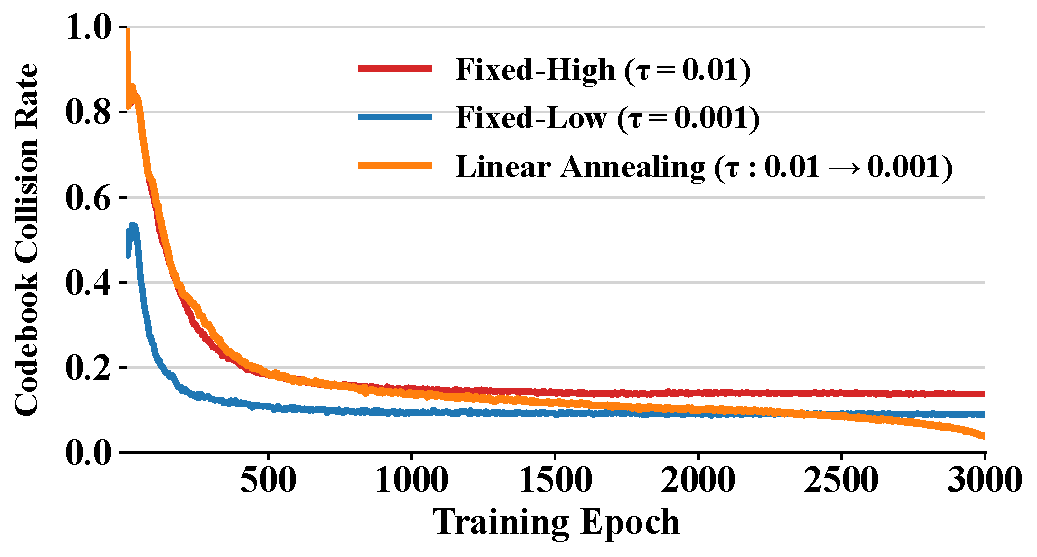
\includegraphics[width=0.9\columnwidth]{figure/annealing_ablation_collision_curve.manual.pdf}
    \caption{Results of the collision rate curves during training under different temperature ($\tau$) schedules.}
    \label{fig:annealing}
\end{figure}

\subsubsection{Impact of Temperature Annealing Design}
To address the \textit{Training–Inference Discrepancy}, we propose an \textit{Annealed Inference Alignment} strategy that linearly decays the temperature $\tau$ from 0.01 to 0.001. We compare this strategy against two fixed-temperature baselines: Fixed-High ($\tau=0.01$) and Fixed-Low ($\tau=0.001$). We then analyze the codebook collision rate, which is defined as one minus the ratio of the number of unique hard identifiers to the total number of items, over the course of training for each strategy.

The results are summarized in Figure~\ref{fig:annealing}. Fixed-Low maintains a lower collision rate than Fixed-High due to harder assignments, while Fixed-High remains consistently high. Our annealed strategy starts similar to Fixed-High, allowing gradient flow and semantic exploration, then gradually decreases and ultimately falls below Fixed-Low. This shows that annealed inference alignment enables both early exploration and minimal codebook collisions, effectively bridging the training–inference gap.

\begin{figure}[t]
    \centering
    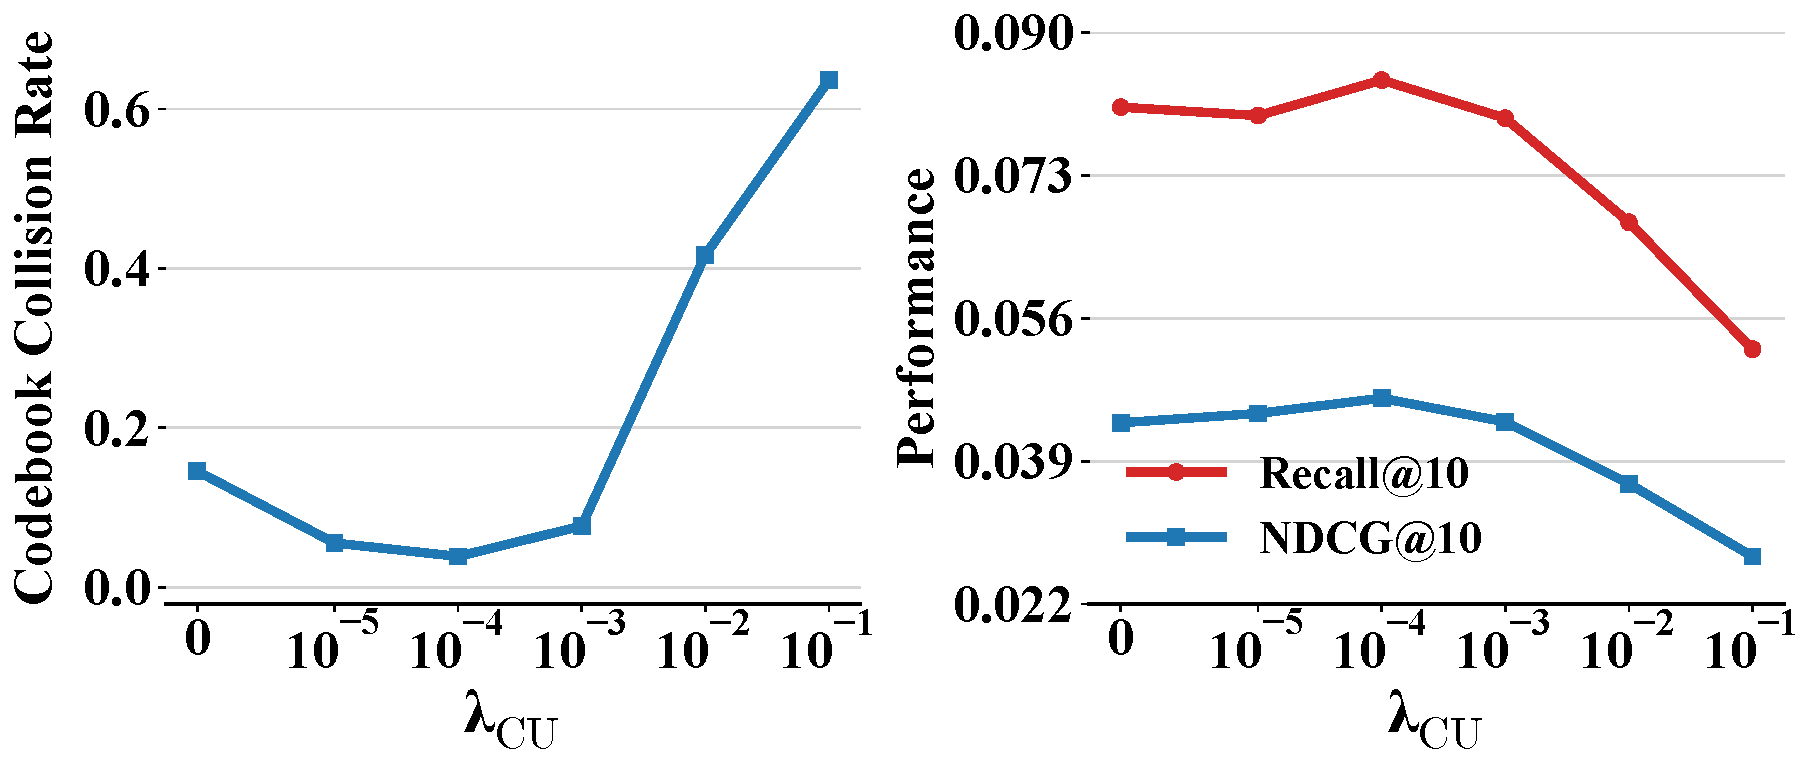
\includegraphics[width=\linewidth]{figure/diversity_ablation_collision_vs_lambda.manual.pdf}
    \caption{Results of the collision rate and recommendation performance of UniGRec across different values of the uniformity regularization weight ($\lambda_\text{CU}$). }
    \label{fig:diversity}
\end{figure}

\subsubsection{Impact of Hyperparameter $\lambda_{\text{CU}}$}

To mitigate \textit{Item Identifier Collapse}, we introduce \textit{Codeword Uniformity Regularization} ($\mathcal{L}_\text{CU}$) and vary its weight $\lambda_{\text{CU}}$ over $[0, 10^{-5}, \dots, 10^{-1}]$, measuring the resulting codebook collision rate and recommendation performance.

Figure~\ref{fig:diversity} shows a strong negative correlation between codebook collision rate and recommendation accuracy. As $\lambda_\text{CU}$ increases from $0$ to $10^{-4}$, collisions are effectively reduced, resulting in peak performance and confirming that a more balanced codebook enhances item differentiation. However, when $\lambda_\text{CU}$ exceeds $10^{-2}$, excessive regularization causes collisions to rise sharply and performance to decline, likely due to disruption of the semantic embedding reconstruction process.

\subsection{In-Depth Analysis (RQ4)}
\label{sec:analysis}

\begin{figure}[t]
  \centering
  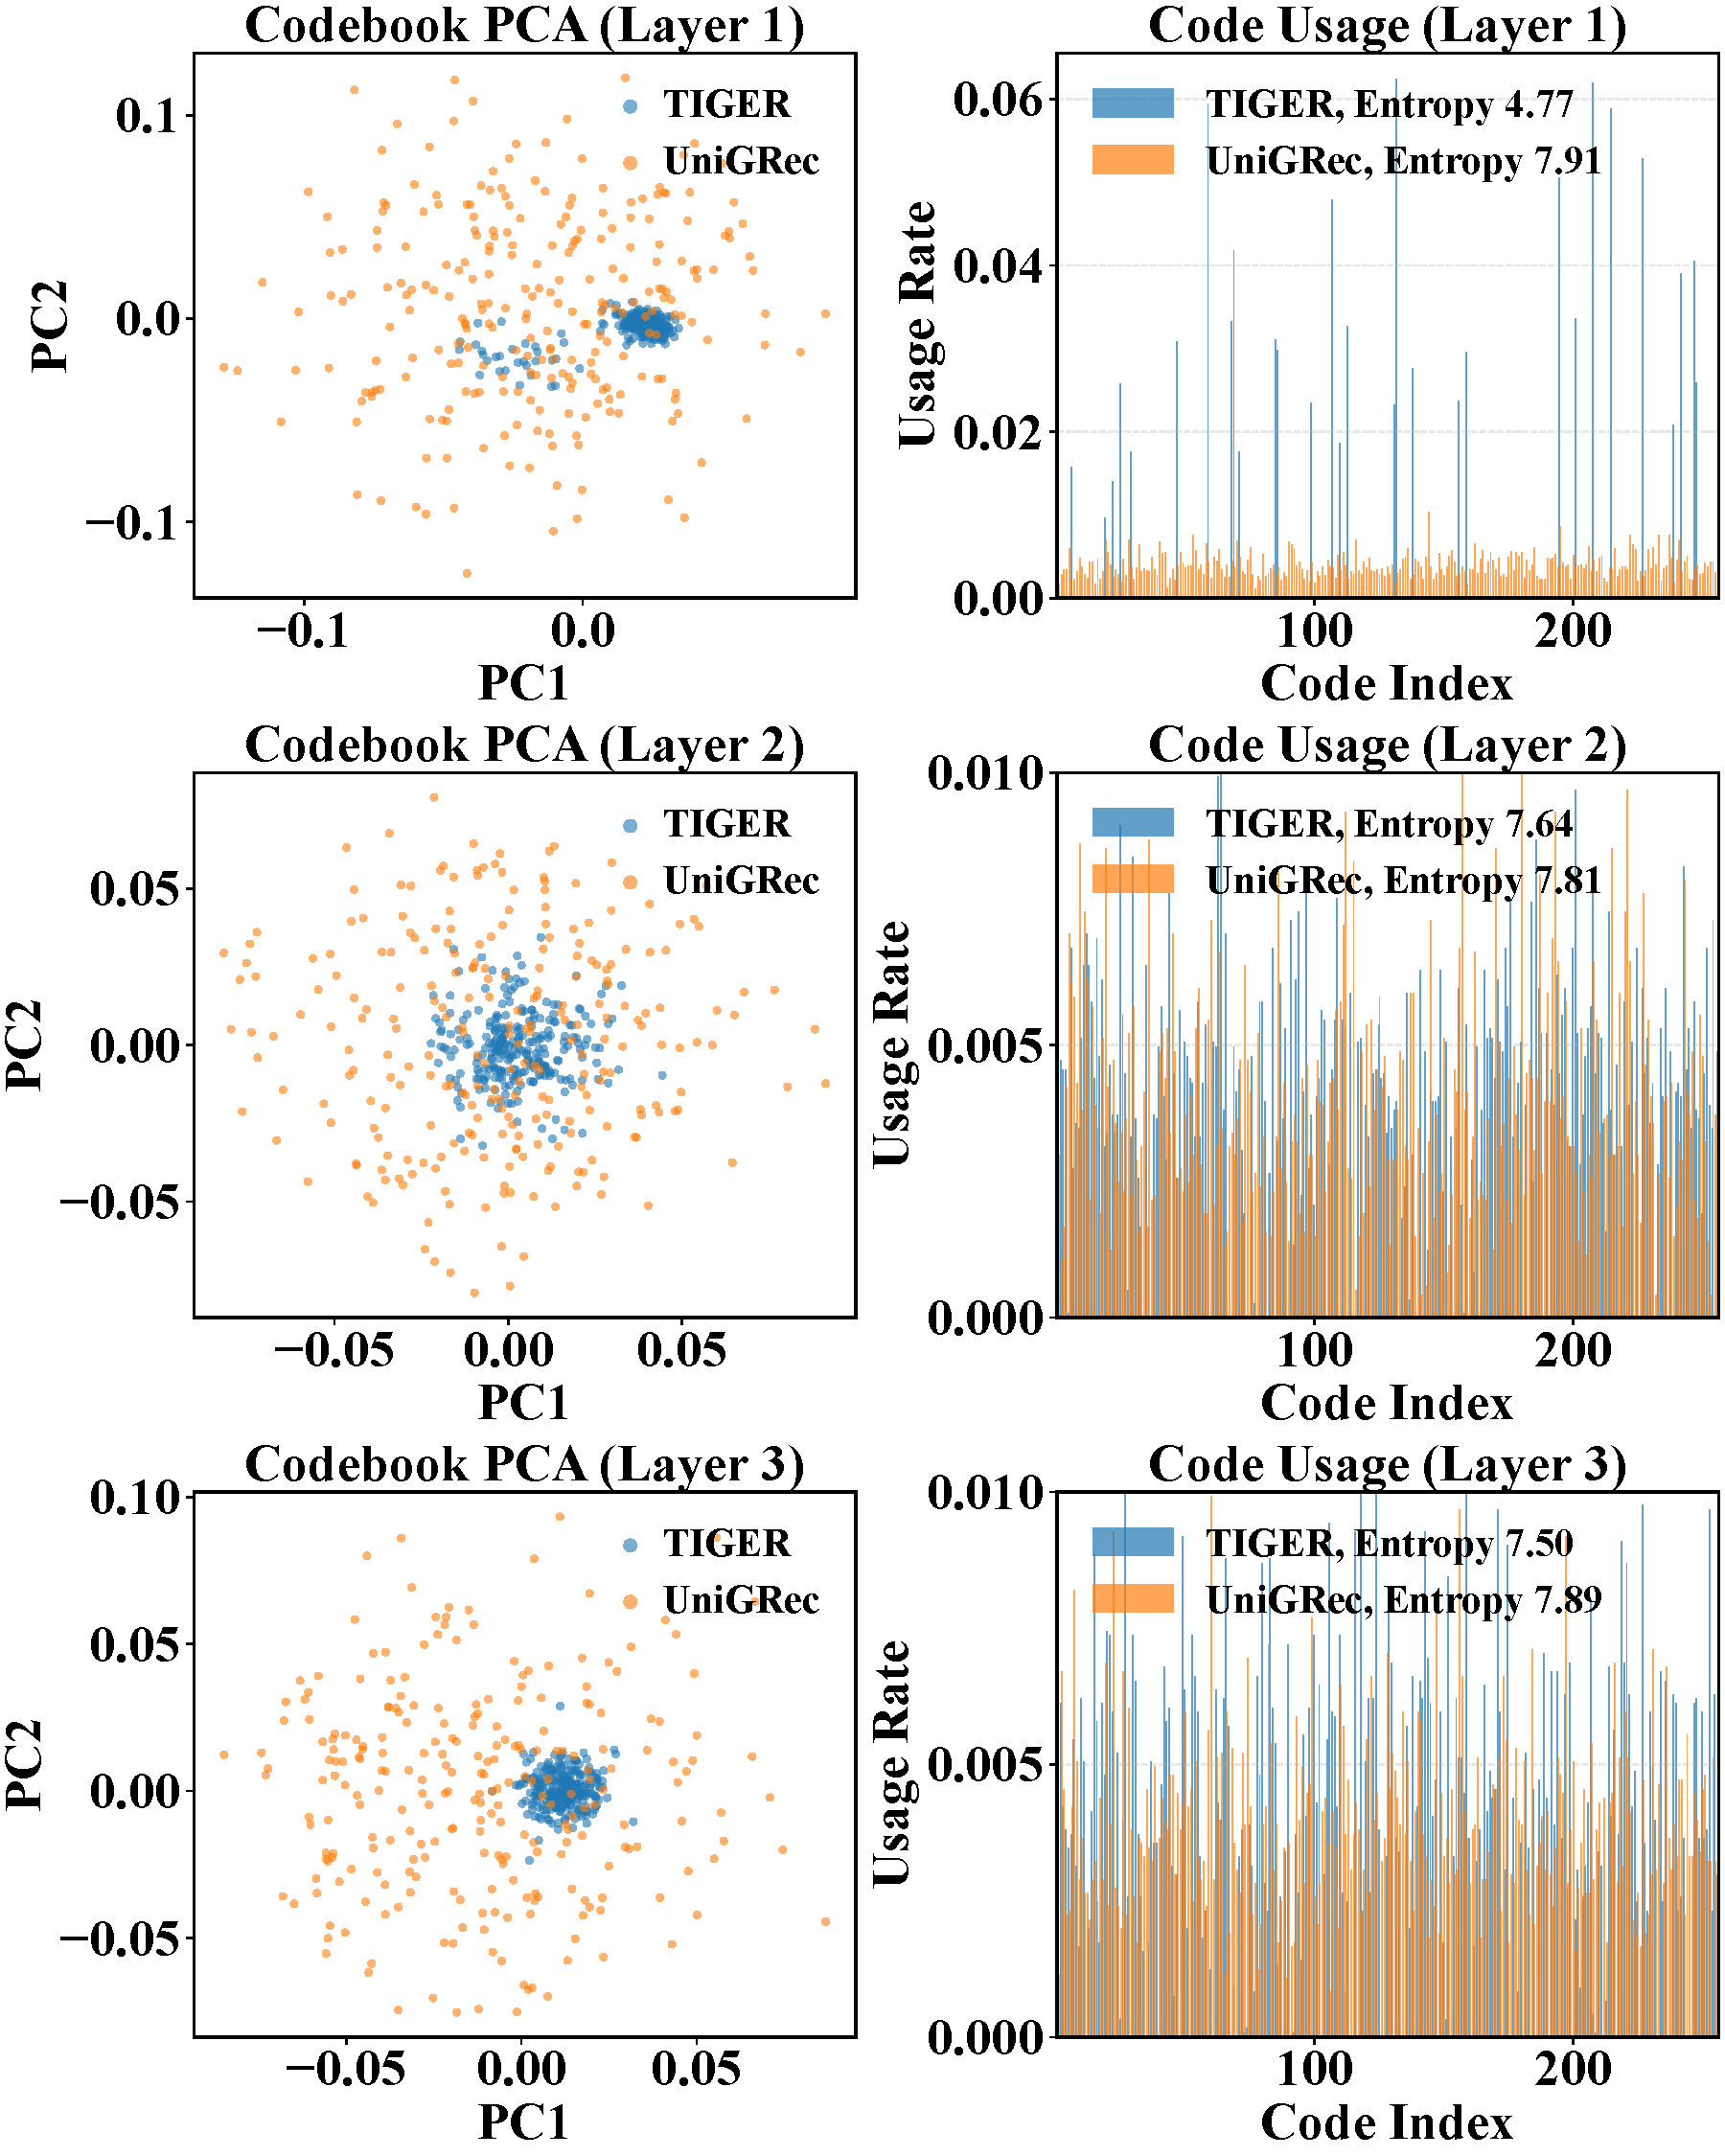
\includegraphics[width=\linewidth]{figure/pca_and_usage_all_layers.pdf}
  \caption{Visualization analysis of codebook embeddings and codeword usage of each quantization layer, where “Entropy” measures the distribution of codeword usage, indicating how evenly the codewords are utilized.}
  \label{fig:codebook_analysis}
\end{figure}

Finally, we conduct a detailed analysis to understand the sources of improvement and identify the specific changes responsible for the observed gains.

\subsubsection{Codebook Analysis}
We examine the codeword embeddings across the three layers of the codebook. For each layer, we apply PCA to reduce the embeddings to two dimensions for visualization. In addition, we analyze codeword usage across all items based on their hard identifiers, computing the entropy to quantify how evenly the codewords are utilized. For comparison, we include results for TIGER, which serves as an ablated version of our framework with all specialized design components removed.

The results, summarized in Figure~\ref{fig:codebook_analysis}, reveal clear differences between the methods. From the perspective of representation, UniGRec exhibits a widely dispersed, isotropic distribution that effectively spans the latent space, indicating a more expressive semantic space where items are mapped to distinct identifiers that are easier for the recommender to differentiate. From the perspective of utilization, UniGRec achieves a near-uniform codeword distribution with substantially higher entropy, whereas TIGER concentrates usage on a few dominant codewords. These findings demonstrate that our method effectively mitigates codebook collapse and maximizes representational capacity.

\subsubsection{Identifier Analysis}

After analyzing the differences between UniGRec and TIGER at the codebook level, we further investigate the training dynamics of UniGRec by examining how item identifiers evolve across the two training stages (\ie, stage~1 and stage~2 described in Section~\ref{sec:pipeline}). For clarity, we focus on hard identifiers, which are derived from the corresponding soft identifiers. We extract the identifiers of all items after stage~1 and stage~2 training, respectively, and conduct a statistical analysis from two perspectives. First, we measure the proportion of identifier changes at each layer. Second, from an item-level perspective, we analyze the change patterns, \ie, which layers of an item’s identifier are modified.

The results are summarized in Figure~\ref{fig:case_study}, from which we draw the following observations:
\begin{itemize}[leftmargin=*]
\item \textbf{Layer-level analysis.} The change rate remains relatively stable and low overall, and gradually decreases with increasing layer depth, which aligns with the design principle of residual quantization. This suggests that joint training refines item identifiers in a coarse-to-fine manner.
\item \textbf{Item-level analysis.} Over 93\% of items exhibit changes in at most one layer or remain unchanged. This indicates that end-to-end joint training acts as a recommendation-aware fine-tuning of the tokenizer rather than a disruptive retraining. Consequently, from the tokenizer perspective, the observed performance gains can be attributed to two complementary factors: the transition from hard to soft identifiers and the recommendation-aware refinement of item identifiers.
\end{itemize}

\begin{figure}[t]
  \centering
  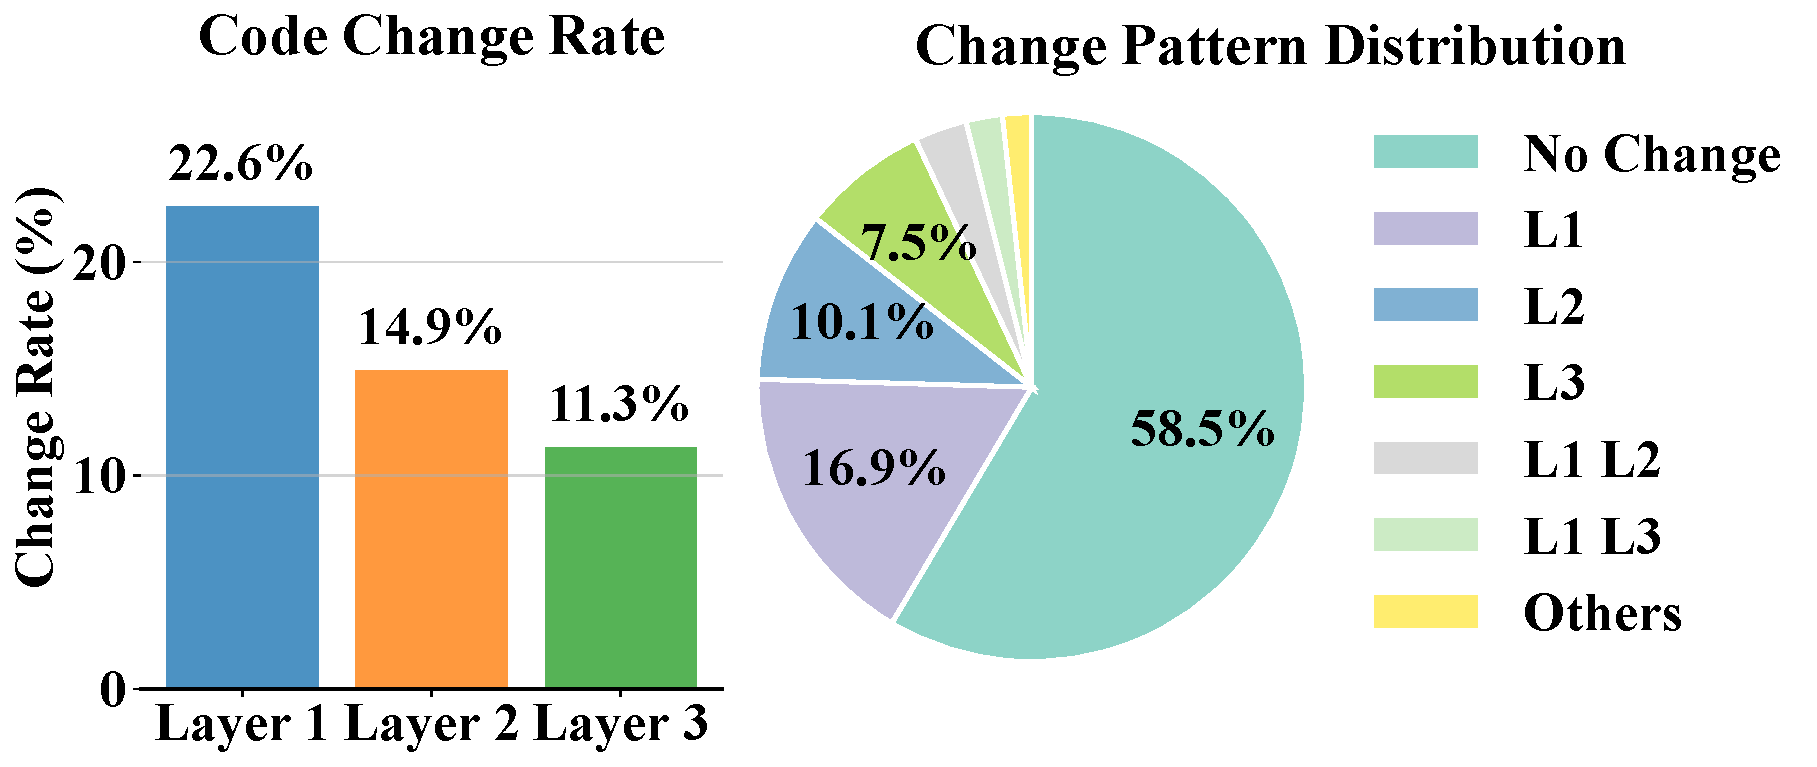
\includegraphics[width=\linewidth]{figure/case_study_code_change_analysis.pdf}
  \caption{Analysis of identifier evolution, including the code change rate across layers and the distribution of identifier change patterns.}
  \label{fig:case_study}
\end{figure}
